\section{Design of XXX}
\label{sec:design}
\begin{figure}[t]
  \centering
  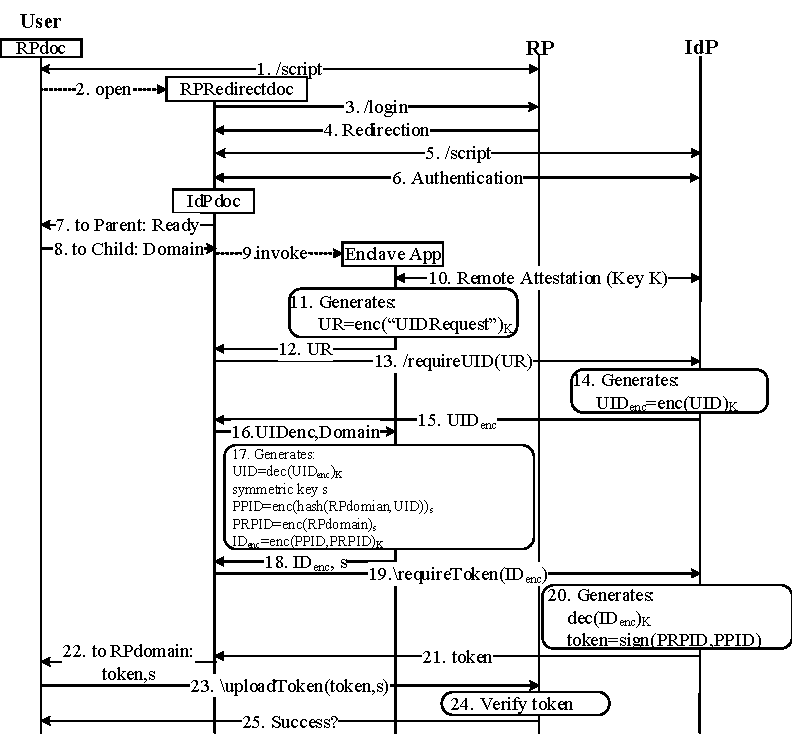
\includegraphics[width=\linewidth]{fig/sgx-sso.pdf}
  \caption{The protocol flow of XXX.}
  \label{fig:XXX}
\end{figure}
The XXX is compatible with OIDC, besides that the IdP service is separated into user agent part and server part. 
The server part IdP service takes the responsibility of authenticating the user, retrieves the UID for each user, and issues the signed identity proof consisted the privacy-preserving RP and user identifier generated at user agent part IdP service.
The user agent part IdP service would obtain the UID from server part service, transform UID into the PPID, and encrypt the RPID and PPID with an one-time symmetric key to avoid IdP server digging out the RP's identity. As the enclave application is protected by SGX, it must not conduct any malicious behaviour. 

\subsection{XXX process}
In this section, we provide the detail protocol of XXX.

The process of XXX is depicted in detail in Figure~\ref{fig:XXX}.
The SSO process is started with the user's visit to an RP at her browser, and the browser downloads the RP script (step 1), which is used to conduct the behaviour defined by RP at user side. Then the RP script opens the new window with the RP login endpoint (step 2, 3). Then the user is redirected to the IdP server (step 4). It must be noticed that, the user cannot visit IdP at step 2,3 directly because of the $Referer$ attribute in HTTP header. While the script in origin A opens a new window with origin B, the HTTP request to B will carry the key value $Referer: A$. Therefore, the RP's domain is exposed to IdP. With HTML5, a special attribute for links in HTML was introduced, that the $ref="noreferrer"$ can be used to make $Referer$ header be suppressed. However, when such a link is used to open a new window, the new window does not have a handle on the opening window (opener) anymore. The handle is necessary for XXX to transmit messages between RP and IdP.



While the user is redirected to the IdP server, the IdP will retrieve the IdP script (step 5), witch is used to deal with the interaction with IdP server, RP script and enclave application.
And the IdP authenticates the user (step 6). After the IdP script is downloaded, it sends the ready signal to its opener (i.e., the RP window) (step 7). Then it will receive the $RPdomain$ from RP script for further process (step 8). There are some types of parameters required in OIDC protocol to be carried in the SSO request, such as $response\_type$ and $scope$. In this paper, we would not focus on these attributes, and only describe the necessary parameters. 

Then the IdP script invokes the enclave application (step 9). The enclave application conducts remote attestation at its initialized execution (step 10). After the remote attestation, enclave application and IdP server shares a symmetric key $K$. 

The enclave application generates the $UID$ request (i.e., $UR$) by encrypted request information with $K$ (step 11), and return it back to IdP script (step 12). Then the user starts the $UID$ request to IdP (step 13). IdP encrypts $UID$ with $K$ (step 14) and sends it to user (step 15). 


While IdP script receives the encrypted $UID$, it transmits it to enclave application with RP's domain (step 16). The enclave application derives the $UID$ with $K$, generates the symmetric key $s$, encrypts the RP's domain with key $s$ as the transformed RP ID (i.e., $PRPID$), encrypts the hash of RP's domain and UID as the $PPID$, and encrypts $PRPID$ and $PPID$ with $K$ (step 17). After the ID transformation, enclave application sends the encrypted IDs and $s$ to IdP script (step 18).


Then user sends the encrypted $PRPID$ and $PPID$ to IdP for identity token (19). 
The IdP server derives the $PRPID$ and $PPID$, signs the $token$ consisted of $PRPID$ and $PPID$ as the identity proof (step 20), and returns it to enclave application (step 21). 
The IdP script then sends the $token$ and $s$ to the origin $RPdomain$ through $postMessage$ (step 22). It guarantees that only the script running in the RP window can receive the $token$, which avoids the man-in-the-middle attack.

Finally, the RP script uploads the $token$ and key $s$ to RP server (step 23). The RP server firstly verifies the signature with IdP's public key, then generates the $PRPID$ with its domain and key $s$, and compared it with the one carried by $token$. If the two $PRPID$s are equal, RP decrypts the user's ID from $PPID$, and find out the related user information in its database (step 24). Then it returns the login result to user (step 25). 